\documentclass{bioinfo}
\usepackage{url}

\usepackage[british,english]{babel}
\usepackage{mathpazo}
\usepackage{color}
\definecolor{deepblue}{rgb}{0,0,0.5}
\definecolor{deepred}{rgb}{0.6,0,0}
\definecolor{deepgreen}{rgb}{0,0.5,0}

\usepackage{listings}
\usepackage{setspace}

\definecolor{Code}{rgb}{0,0,0}
\definecolor{Decorators}{rgb}{0.5,0.2,0.2}
\definecolor{Numbers}{rgb}{0.5,0,0}
\definecolor{MatchingBrackets}{rgb}{0.25,0.5,0.5}
\definecolor{Keywords}{rgb}{0,0.6,0}
\definecolor{self}{rgb}{0,0,0}
\definecolor{Strings}{rgb}{0.6,0.2,0}
\definecolor{Comments}{rgb}{0,0.63,1}
\definecolor{Backquotes}{rgb}{0,0,0}
\definecolor{Classname}{rgb}{0,0,0}
\definecolor{FunctionName}{rgb}{0,0,0}
\definecolor{Operators}{rgb}{0,0,0}
\definecolor{Background}{rgb}{1,1,1}
\definecolor{Modules}{rgb}{0,0,0.8}

\lstnewenvironment{python}[1][]{
\lstset{
%numbers=left,
numberstyle=\footnotesize,
numbersep=1em,
xleftmargin=0em,
framextopmargin=2em,
framexbottommargin=2em,
showspaces=false,
showtabs=false,
showstringspaces=false,
%frame=l,
tabsize=4,
% Basic
basicstyle=\ttfamily\footnotesize\setstretch{1},
backgroundcolor=\color{Background},
language=Python,
% Comments
commentstyle=\color{Comments}\slshape,
% Strings
stringstyle=\color{Strings},
morecomment=[s][\color{Strings}]{"""}{"""},
morecomment=[s][\color{Strings}]{'''}{'''},
% keywords
morekeywords={import,from,class,def,for,while,if,is,in,elif,else,not,and,or,print,break,continue,return,True,False,None,access,as,del,except,exec,finally,global,import,lambda,pass,print,raise,try,assert},
keywordstyle={\color{Keywords}\bfseries},
% additional keywords
morekeywords={[2]@parametric},
keywordstyle={[2]\color{Decorators}\slshape},
emph={self},
emphstyle={\color{self}\slshape},
%
}}{}


\usepackage[T1]{fontenc}
% \usepackage[latin9]{inputenc}
\usepackage{float}
\usepackage{amsmath}
\usepackage{graphicx}
\usepackage{setspace}
\usepackage{amssymb}
\usepackage{natbib}
\usepackage[title]{appendix}
\usepackage{siunitx}
\usepackage{chngcntr}
\usepackage{algorithmic}
\renewcommand{\algorithmicrequire}{\textbf{Input:}}
\renewcommand{\algorithmicensure}{\textbf{Output:}}

\usepackage{multirow}
\usepackage{rotating}
\usepackage{hyperref}

\makeatletter
\newfloat{algorithm}{H}{loa}[section]
\floatname{algorithm}{Algorithm}
\counterwithout{algorithm}{algorithm}
\def\argmin{\mathop{\operator@font arg\,min}} 
\def\argmax{\mathop{\operator@font arg\,max}} 
\makeatother

\copyrightyear{}
\pubyear{}

\begin{document}
\firstpage{1}

\title[DIPY]{Dipy, a library for the analysis of diffusion MRI data}

\author[Garyfallidis, Brett, Amirbekian, Rokem,  van der Walt, Descoteaux, 
Nimmo-Smith]{Eleftherios~Garyfallidis\,$^{1,2,*}$, Matthew~Brett\,$^{3}$,
  Bago~Amirbekian\,$^{4}$, Ariel~Rokem\,$^{5}$, Stefan~van der Walt\,$^{7}$, Maxime~Descoteaux\,$^{2}$, Ian~Nimmo-Smith\,$^{6}$ and Dipy~Contributors $^{8}$\footnote{to whom correspondence should be addressed. e-mail: garyfallidis@gmail.com}}

\address{\,$^{1}$University of Cambridge, Cambridge, UK\\
  \,$^{2}$University of Sherbrooke, Sherbrooke, CA\\ 
  \,$^{3}$University of California, Henry H. Wheeler, Jr. Brain Imaging Center, Berkeley, CA.\\
  \,$^{4}$University of California, San Francisco, CA, USA\\    
  \,$^{5}$Stanford University, Stanford, CA, USA\\
  \,$^{6}$MRC Cognition and Brain Sciences Unit, Cambridge, UK\\
  \,$^{7}$Stellenbosch University, Stellenbosch, South Africa\\
  \,$^{8}$http://dipy.org/developers.html  
  }

\history{}

\editor{}

\maketitle

\begin{abstract}
\noindent

Diffusion Imaging in Python (Dipy) is a free and open source software
project for the analysis of data from diffusion magnetic resonance
imaging (dMRI) experiments. DMRI is an application of MRI that can be
used to measure the micro-structure of the white matter in the human
brain \emph{in vivo}. It utilizes pulsed directionally oriented
magnetic gradients to estimate diffusion in different directions and
locations in the brain non-invasively. Many methods have been developed
to model the local configuration of nerve fibers in the white matter
based on this information and to infer the trajectory of nerve fascicles
connecting different parts of the brain. 

Dipy gathers implementations  of many different methods, where they can be easily understood and compared. Dipy aims to provide transparent implementations for all the different steps of dMRI analysis with a uniform API. We have implemented classical signal reconstruction techniques, such as the diffusion tensor model and deterministic fiber tractography. In addition, it implements cutting edge novel reconstruction techniques, 
such as constrained spherical deconvolution and diffusion spectrum imaging with deconvolution, as well as methods for probabilistic tracking and unique methods for tractography clustering. Many additional utility functions, to calculate various statistics of dMRI data, visualization functions, as well as file-handling routines exist to assist in the development and use of novel techniques.
 
In contrast to many other scientific software projects, dipy is not being developed by a single research group. Rather, it is an open project that encourages contributions from any scientist/developer through the github Pull Request mechanism and open discussions on github and on the project mailing list. Consequently, dipy has today an international team of contributors, spanning 6 different academic institutions in 4 countries and 3 continents, and still growing (http://dipy.org).

\section{Keywords:} Python, Diffusion MRI, Diffusion Tensor,
Spherical Deconvolution, Medical imaging, Free Open Source Software, Deterministic
tractography, Probabilistic tractography, Fiber tracking, Medical Visualization.

\end{abstract}

\section{Skeleton}
Here is a possible outline for the paper:
\begin{verbatim}
Introduction
Philosophy/Mission
General Design Aspects
How we work (git/github etc)
File Formats 
Preprocessing
   Load/Save data
   Mask the background
Reconstruction
   DTI 
   DSI
   QBall
   Spherical Deconvolution 
Tracking
   Deterministic
   Probabilistic
Post-tracking
   Segmentation
   Track\_counts
   Track Lengths & other statistics
   Connectivity matrix
Discussion/Conclusions
\end{verbatim}

\section{Introduction}

\emph{Diffusion MRI} (dMRI) \citep{stejskal-tanner:65,
  lebihan-breton:85,merboldt-hanicke-etal:85, taylor-bushell:85, callaghan:91}
is an MRI technique that provides information about the structure of neuronal pathways found in the white matter and other body tissue with fiber-like structure. DMRI acquires one or more $T_{2}$ reference images, and a collection of diffusion-weighted images, in which $T_{2}$ signal is attenuated according to the  diffusivity of water along prescribed gradient directions \citep{behrens-johansen-berg:09, jones:10}.

Because of its unique capability to characterize the micro-structure of neural tissue, and the inferences that can be made using this information about structural connectivity dMRI has had increasing popularity, with more than five thousand papers published according to PubMed only for 2012. This popularity is also evident from the large number of software tools available for the analysis of diffusion-weighted images. Many of these tools are written in C/C++: 3D Slicer \citep{pieper:06}, AFNI \citep{cox-afni:12}, MITK \citep{fritzsche-mitk:12}, BrainVoyager QX \citep{goebel-brainvoyager:12}, DTI-Query/Quench \citep{sherbondy:05}, FreeSurfer \citep{fischl-freesurfer:12}, FSL-FDT \citep{smith-fdt:04}, MedInria \citep{toussaint-souplet-etal:07}, MRtrix \citep{Tournier2012}, Diffusion Toolkit/Trackvis \citep{wang-diffusion-toolkit:07}, FiberNavigator \citep{vaillancourt:11, chamberland:13}. Only a few are written in other languages, such as R: TractoR \citep{ clayden-TractoR:11}, Java: Camino \citep{Cook2006} and Matlab: ExploreDTI \citep{leemans-exploredti:09}, AFQ \citep{yeatman2012afq} and others.

Dipy (\textit{Diffusion Imaging in Python}) is the first collective effort to create an open-source diffusion MRI analysis library using the Python language. Python is a general purpose, object-oriented programming language which was designed with an emphasis on code readability. This emphasis allows scientists who are not trained as software engineers to understand the computational steps taken in analysis and extend the software in a straight-forward manner. Being an interpreted language, Python does not require additional compilation, linking, etc. and so installation of software written in Python is relatively easy. Taken together, these properties of the language are powerful assets for the design of the next generation of medical imaging analysis tools. In the past we found that many researchers were using available tools without understanding the underlying details, often because the details were hidden from the users. Dipy tackles this problem by being free, open source (BSD license), simple and well documented. In addition, the recent explosion of Python users, the many Python tools for scientific computing \citep{perez_python:11}, \citep{mckinney_python:12}, \citep{perez_ipython:07} and the recent stack of neuroimaging\footnote{\url{http://nipy.org}} modules make Dipy a nice addition for those who prefer Python as their favorite language.

Dipy takes advantage of the growing ecosystem of tools written for scientific computing in Python. It is built on top of production-ready high-performance Python libraries. Primarily, Dipy depends on Numpy\footnote{\url{http://numpy.org}}. The core structure of this library is an implementation of an Array \citep{van_numpy:11} class. Numpy arrays are used for representation of numerical data in Python and enable efficient implementation of numerical computations, such as vectorized computations, avoiding copying data in memory, and minimizing operations. Numpy is also used for matrix, tensor and linear algebra operations.  Dipy further depends on Scipy\footnote{\url{http://scipy.org}} for nonlinear optimization and other volumetric operations. Cython\footnote{\url{http://cython.org}} is used in rare cases when both standard Python and Numpy/Scipy are not efficient enough for the task at hand. Cython interprets Python code into plain C performance by adding static type declarations. The last absolute dependency for Dipy is Nibabel\footnote{\url{http://nipy.org/nibabel}} which is used for loading and saving medical imaging file formats.

Optional dependencies, that are not required for analysis, are used for visualization of diffusion data and the results of analysis. Matplotlib\footnote{\url{http://matplotlib.org}} is used for 2D and 3D plotting. In addition, Python-VTK\footnote{\url{http://vtk.org}} is used for more advanced 3D interactive visualization. Furthermore, we recommend using IPython\footnote{\url{http://ipython.org}} the interactive Python shell for calling and debugging our scripts. 

In the following sections, we will explain the philosophy and main design concepts behind Dipy. We will also give examples which cover different parts of the diffusion MR analysis pipeline from the local voxel reconstruction of orientation distribution functions to streamline generation and visualization. 

\section{Philosophy and Mission}

Mission: The purpose of Dipy is to make it easier to do better diffusion MR imaging research. We aim to build software that is clearly written, clearly explained, well tested, a good fit for the underlying ideas and a natural home for collaboration.

Dipy is a true international project where everyone from anywhere in the world is welcome to contribute as long as they agree with our mission statement. In order to be faithful to our mission we all have to follow specific policies. For example, lets assume that a scientist makes a nice new discovery and wants to share some code. Even if the discovery is of substantial importance the code will not be included in the main project without extended testing from the main author and code reviews from other members of the team. For the code reviews we make sure that at least two developers. In that way we make sure that quality assurance is kept at the highest level. 

Using this work ethic Dipy has managed to grow into an international and multi-departmental team of highly skilled contributors from different levels of education (Master students, PhD students, Post-Docs and Professors) spanning the fields of Computer Science, Medicine, Applied Mathematics, Biomedical Engineering and Psychology. 


\section{Terminology}

As in many other fields of science, dMRI is a field that uses specific terminology to describe the constructs of the measurement, as well as to describe the interpretation of the results of the analysis. We rely on a recent paper \citep{Cote2013tractometer}, that has proposed specific terminology for describing different constructs of the dMRI field. In this section we will describe constructs of the measurement, as well as constructs used to interpret the results of the analysis. We will use this terminology to explain the analysis code and interpretation of data in subsequent sections. 

The measurement of dMRI data relies on the application of a pulsed magnetic gradient and the degree of sensitization to diffusion depends on a number of parameters, including the duration of the gradient, time that elapses between pulses of the gradient and the gradient amplitude. These parameters are together summarized in what is referred to as the "b-value".  As described above, the measurement is conducted in several different directions and these are encoded in so-called "b-vectors". These are unit vectors that describe the direction relative to the scanner coordinate frame in which the gradients are applied. Different algorithms are used to determine the placement of these b vectors (e.g. \citep{jones-etal:99}).

While we are ultimately interested in the identification of the trajectories of bundles of axons, which are the long fiber-like part of a nerve cell along which electrical impulses are conducted from cell to cell (and whose size is on the $\mu$m scale), the measurement is conducted on a much larger scale. Typically, the measurement is conducted in a grid of "voxels" of approximately 2x2x2 mm. We are therefore limited to describe the trajectories of "fascicles" of nerves. One of the major achievements of this field is that it is now possible to reliably and accurately identify major fascicles in individual experimental participants or patients. These major fascicles are also known as "tracts". This is a term taken from neuroanatomy and describes a group of neuronal axons within the central nervous system (mm scale). 

For the purpose of interpretation of these data, a "fiber" can be any long and thin structure. Hence, fiber tracking is a general term that can be used in any field that reconstructs fibrous structures, such as hair fibers, celery fibers, muscle fibers, prostate fibers, brain fibers, etc. "Fiber bundles" denote groups of fibers usually with an anatomical or functional meaning. These can be major tracts in the brain, such as the arcuate fasciculus, which connects parts of the posterior temporal lobe with the frontal lobe, the fornix, which connects the medial temporal lobe with sub-cortical structures, such as the hypothalamus and amygdala,  etc. A fiber bundle for the area of brain anatomy is synonymous to a tract, also often called fiber tract. The term tract can be misleading when talking for example about the corticospinal tract, because the corticospinal tract is in fact not a single tract but a group of tracts (including corticobulbar projections, the pyramidal tract, etc.).

Tractography is the computational process through which the fibers are detected and delineated. Tractography relies on the assumption that diffusion of water, as reflected in the dMRI measurement, occurs more freely along the axis of an axon, than across the membranes of the axon. Tractography is therefore usually done by by finding the directions of diffusion in each voxel (see 'Reconstruction', below) and stepping through the brain volume along the directions of large diffusion estimated in each location. This process generates so-called streamlines, which imaginary lines that approximate the underlying fiber. Streamlines are also sometimes referred to as "tracks". These are not to be confused with tracts: While a tract is a physical object, a track is a computational construct that only approximates the underlying fascicle or bundle of fibers. Confusingly enough "streamline bundles", or simply "bundles" are often used to refer to a group of streamlines with similar shape and spatial characteristics. These do not necessarily correspond to individual physical fiber bundles but are instead also computational constructs that approximate the underlying anatomy.


\section{General design aspects}

API (module diagram), Git/Github, continuous integration, sphinx for documentation, nosetests for testing

Need a diagram with the base (numpy, nibabel) and the rest of the modules on top.

Dipy contains the following modules

\tiny
\begin{verbatim}
| modules       | main usage                | sub-modules                        |
| ------------- | ------------------------- | ---------------------------------- |
| reconst       | reconstruction modules    | dti, dsi, csd, odf, shm, gqi       |
| tracking      | tractography algorithms   | EuDX, Modular tracking (det, prob),|
|               |                           | distances, metrics, utils          |
| core          | general usage functions   | spheres, gradients, electrostatics,|
|               |                           | geometry, ndindex                  |       
| viz           | 2D/3D visualization       | fvtk, 2D sphere plots, colormaps   |
| io            | input/io utilities        | pickles, gradients, dpy(HDF5)      |
| external      | other software            | fsl                                |
| align         | alignment, reslicing      | aniso2iso                          |
| sims          | voxel & volume simulations| voxel, phantom                     |
| data          | small data & online data  | fetcher                            |
| segment       | clustering & segmentation | quickbundles                       |

There are also some command line scripts in dipy/bin and many tests.
\end{verbatim}
\normalsize

\begin{python}
import dipy
dipy.__version__
'0.7.0.dev'
\end{python}

\section{Preprocessing}

\subsection{Load/Save data}
The most basic operation that we do in Neuroimaging is to load some data from the disk which are often extracted from an MRI scanner. Surprisingly this is often a difficult task as different scanners and software read/write the data in different ways. Nibabel a library for reading medical imaging formats is coming here to the rescue supporting ANALYZE (plain, SPM99, SPM2), GIFTI, NIfTI1, MINC, MGH, ECAT, PAR/REC, Freesurfer(geometry, morphometry files) and with a growing support for DICOM. 

The most common file format used in dMRI is the NifTI1. Assuming that we have a file with our 4D raw diffusion data we can load it in the following way.
\begin{python}
fimg = "raw.nii.gz"
import nibabel as nib
img = nib.load(fimg)
\end{python}
\texttt{fimg} holds the filename for the file, \texttt{nib} is a shortcut for the Nibabel module, \texttt{img} is an object that Nibabel creates which contains all the information from the file e.g. the header, the 3D data and the affine. We can obtain all these using \texttt{get} methods.
\begin{python}
data = img.get_data()
affine = img.get_affine()
header = img.get_header()
voxel_size = header.get_zooms()[:3]
\end{python}
The \texttt{data} is an Numpy array which contains the actual 4D image (a collection of 3D volumes). Using \texttt{data.shape} we can obtain the dimensions of the image. In this example the dimensions are (81, 106, 76, 160). The first three dimensions contain the size of the volume and the last dimension has the information for the different diffusion gradients. The variable \texttt{affine} provides a $4\times4$ array which contains the transformation information to go from voxel (image) coordinates to world coordinates (scanner). This can be useful when registering, saving or visualizing images. The \texttt{voxel\_size} is a tuple with 3 values. In this example the \texttt{voxel\_size} is (2, 2, 2) i.e. 2mm cubic.

Lets now assume that we want to extract and save from the 4D data only the first volume which usually is the one without any implied diffusion gradients. This is also known as the S0 (S for signal, and 0 for no gradients). This is very easy using the following code.
\begin{python}
S0 = data[:,:,:,0]
img2 = Nifti1Image(S0, affine)
nib.save(img2, "S0.nii.gz")
\end{python}
As we said \texttt{data} is a Numpy array. Numpy arrays provide simple ways (slicing) to extract information from N-dimensional datasets. For example \texttt{data[10:20, 10:20, 10:20, 30:50]} would give a new sub-array with \texttt{shape} (10, 10, 10, 20). When single column : is used that means that all points in this dimension are used. To save this new array we will need to update the affine. 
\begin{python}
import numpy as np
sub_data = data[10:20, 10:20, 10:20, 30:50]
sub_affine = affine.copy()
sub_affine[:3, 3] += np.array([10, 10, 10])
sub_img = Nifti1Image(sub_data, sub_affine)
nib.save(sub_img, "sub_data.nii.gz")
\end{python} 
For more information about Numpy and slicing have a look at [REFERENCE].

\subsection{Background removal}

\begin{python}
from dipy.segment.mask import otsu_mask
mask = otsu_mask(data[..., 0])
\end{python}

\section{Reconstruction}

In diffusion MRI, the motion of water molecules is probed in a spatial- and direction-specific manner. That is, in every spatial location in the brain (typically sampled in voxels each covering a volume of approximately 2x2x2 mm), the diffusion in several different directions is probed through the application of directional magnetic gradients. Many different models and algorithms have been proposed to describe the full diffusion orientation distribution function (dODF) from these measurements. In addition, the diffusion surface in every voxel is used to infer the spatial geometry of the underlying tissue. This is referred to as the fiber orientation distribution function (fODF, sometimes also referred to as the FOD). Different algorithms to reconstruct the dODF and fODF have different advantages in describing the data and Dipy contains implementations of several of these algorithms. In what follows, we will review the different reconstruction algorithms that are implemented in Dipy and demonstrate the use of these implementations with code examples.  


\subsection{Diffusion Tensor Imaging}

The diffusion tensor model is a model of the dODF. It was first proposed by Basser and colleagues \citep{basser-mattiello-etal:94} and has since been very influential in demonstrating the utility of diffusion MRI in characterizing the micro-structure of white matter tissue. The model relies on the assumption that diffusion is a Gaussian process. Using this assumption the dODF can be modeled with 6 parameters, describing the variance and covariance of the Gaussian diffusion along the three primary axes. From these parameters, several useful measures can be derived: the primary diffusion direction, which in some places in the brain (e.g. in the corpus callosum, the large fiber bundle in the center of the brain that connects the two hemispheres) corresponds to the direction of the white matter fibers in the voxel. Other useful measures quantify the diffusivity along this primary direction and along other directions, as well as the mean diffusivity. The variation in diffusivity along different directions can be. These measures (mean diffusivity, or MD and fractional anisotropy, or FA) are often used to describe the biophysical properties of the underlying tissue. Though many have resorted to describing FA as a measure of "tissue integrity", there is no real basis . Though the density of the tissue and in particular the density of the myelin wrapping the axons in the voxel may affect MD and FA, changes in other factors, such as the dispersion of fiber directions in the voxel crossing may also increase or decrease these measures \citep{wandell-yeatman:13}. Therefore, interpretation of group differences in FA, or longitudinal changes in FA over time should be carefully handled and compared to the results from other modeling techniques.   

That said, these measures are popular among users of dMRI and also quite useful in the sense that behavioral variance in a variety of measures can be predicted based on these measures [REFERENCES?]. Fitting the tensor model and computing univariate statistics from it in Dipy is straightforward. In the following example, we show how the tensor model is fit to data and how univariate measures can be computed.

First, data is loaded into memory, using the nibabel library:
\begin{python}
fimg = "raw.nii.gz"
import nibabel as nib
img = nib.load(fimg)
data = img.get_data()

\end{python}

Next, the b-vectors indicating the directions of the application of gradients in each of the measurements and the b-values indicating the parameters of diffusion sensitization (amplitude of the gradients, their duration, etc.) are read from files that store the values of these parameters:

\begin{python}
fbval = "raw.bval"
fbvec = "raw.bvec"
from dipy.io import read_bvals_bvecs
bvals, bvecs = read_bvals_bvecs(fbval, fbvec)
\end{python}

These parameters are stored in a utility class, created by the $\tt{gradient_table}$ function, which represents the measurement parameters and direction and which is used by the model classes:

\begin{python}
from dipy.core.gradients import gradient_table
gtab = gradient_table(bvals, bvecs)
\end{python}

Next, we can import the diffusion tensor model class and initialize a $\tt{TensorModel}$ class instance: 
\begin{python}
from dipy.reconst.dti import TensorModel
ten = TensorModel(gtab)
\end{python}

Note that at this point in the code no data analysis has occurred yet. Since the analysis of every voxel in the brain will rely on similar infra-structure, the $\tt{TensorModel}$ class instance only sets up this skeleton for the analysis. This same skeleton will be reused for each one of the voxels in the data here, but can also be reused for other data in a similar fashion 

The advantage of this separation of the model and the fit is that [SOMEONE WILL EXPLAIN THIS HERE, BECAUSE HONESTLY, I DON'T UNDERSTAND!!!]. 

Next, we pass the data to the fit method of the . This returns a $\tt{TensorFit}$ class instance which relates to this specific data: 

\begin{python}
tenfit = ten.fit(data)
\end{python}

Once a fit has been conducted, we can compute a variety of derived univariate measures, such as the fractional anisotropy: 

\begin{python}
from dipy.reconst.dti import fractional_anisotropy
fa = fractional_anisotropy(tenfit.evals)
\end{python}


It is common to represent the primary diffusion direction using an RGB representation [REFERENCE?]. The following call does that:
 
\begin{python}
from dipy.reconst.dti import color_fa
cfa = color_fa(fa, tenfit.evecs)
\end{python}

Finally, a few more points about the implementation of DTI. The first is that there is still ongoing research on fitting methods for the tensor model \citep{Koay2006}. Several different methods have been implemented, including non-linear least-squares, ordinary least-squares and weighted least-squares fitting \citep{chung-lu-etal:06}. In addition, there is ongoing research on methods to robustly fit the tensor model, in the face of noisy data \citep{Chang2005, Chang2012}. An implementation of a robust tensor fitting algorithm (RESTORE) is currently in development and should be in the distributed code in version 0.7 of the software. 

The second comment is that many univariate measures have been implemented. Not only can users compute FA, MD and the direction of the principal diffusion direction, but also other statistics that have been proposed in the literature, such as the diffusion linearity, planarity and sphericity \citep{westin:97}, as well as the tensor mode and tensor norm \cite{Ennis2006}

\subsection{Diffusion Spectrum Imaging}

\subsection{QBall Imaging}

\subsection{Constrained Spherical Deconvolution} 

Constrained spherical deconvolution \citep{tournier-calamante-etal:07}, or CSD, is an algorithm for fitting the fiber ODF using a spherical harmonic basis function. Spherical harmonics (SH) are mathematical functions that can be used to construct an orthonormal basis function on the sphere. In analogy to the 1D time-domain, they can be thought of as a Fourier basis set on the surface of the sphere, which can be used to describe any spherical function (such as the dODF and fODF) up to the highest frequency (termed 'order' for SH) of the functions included in the set used as a basis set. Due to their practical mathematical properties, there have been several cases of using spherical harmonics to describe dMRI data, starting from the work of Larry Frank \citep{Frank2001, Frank2002}. CSD applies two major constraints on the fitting of the fODF. The first is that it applies a non-negativity constraint: fODF values that are smaller than 0 are non-physical and are precluded. The other is that CSD applies a sparseness constraint on the fODF - it assumes that only a few of the fODF values will be larger than 0. Applying these two constraints allows fitting the SH basis set up to very high orders - in essence fitting more parameters than data is present. This is known as 'super-resolution'.
 

\section{Fiber tracking}

\subsection{Deterministic}

\subsection{Probabilistic}

\section{Post-tracking}

\subsection{Segmentation}

\subsection{ROIs - streamlines intersections}

Talk about track\_counts.

\subsection{Streamline statistics}

Talk about lenghts and other metrics on streamlines

\section{Discussion/Conclusion}

We have described the Dipy library for analysis of diffusion MRI data. Dipy is a part of the Neuroimaging in Python community (http://nipy.org), a growing community of scientists and developers who are participating in the development of open source software for neuroimaging written in the Python language  . One major source of support for this community comes in the form of the Neurodebian distribution \citep{Halchenko2012}. Neurodebian is a platform for maintenance and deployment of software for the analysis of neuroscience data, based on free open source software (FOSS) practices. 

\section*{Acknowledgments}
Who do we need to acknowledge?

\section*{Disclosure/Conflict-of-Interest Statement}
There are no conflicts of interest.

\section{LaTex Formatting}

This is information for the coauthors of this paper. This section will be removed from the last version of this paper.

This is to show how graphics (EPS) files are included. We use EPS for
speed. The first one is spread across both columns, and the second one
is just in a single column:

\begin{figure*}
\centerline{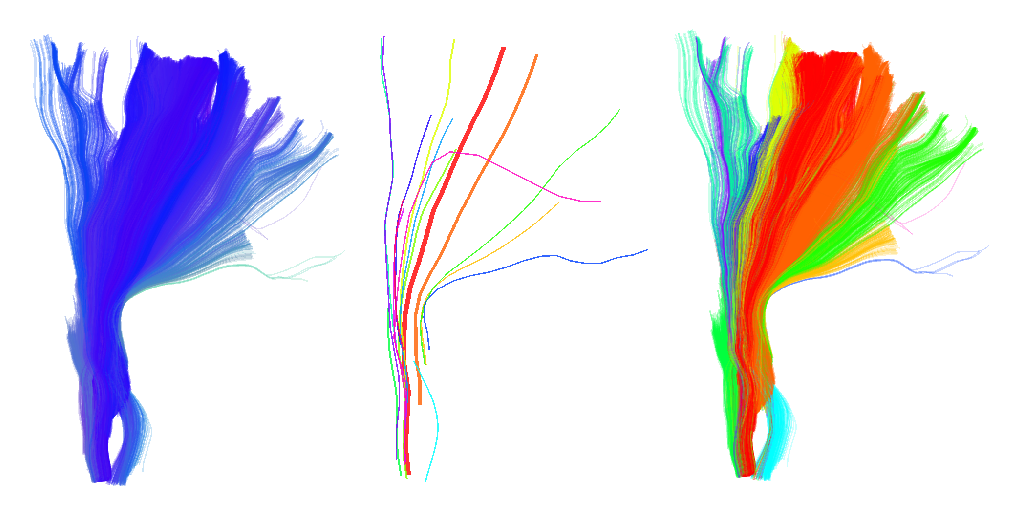
\includegraphics[width=160mm]{Figures/Fig_4_cst_simplification_relabeled_triple.eps}}
\caption{This is the figure caption - and a label to refer to it in the text \label{Fig:big_picture}}
\end{figure*}

When we want to refer to this figure we use the label (see Fig.~\ref{Fig:big_picture}).

\begin{figure}
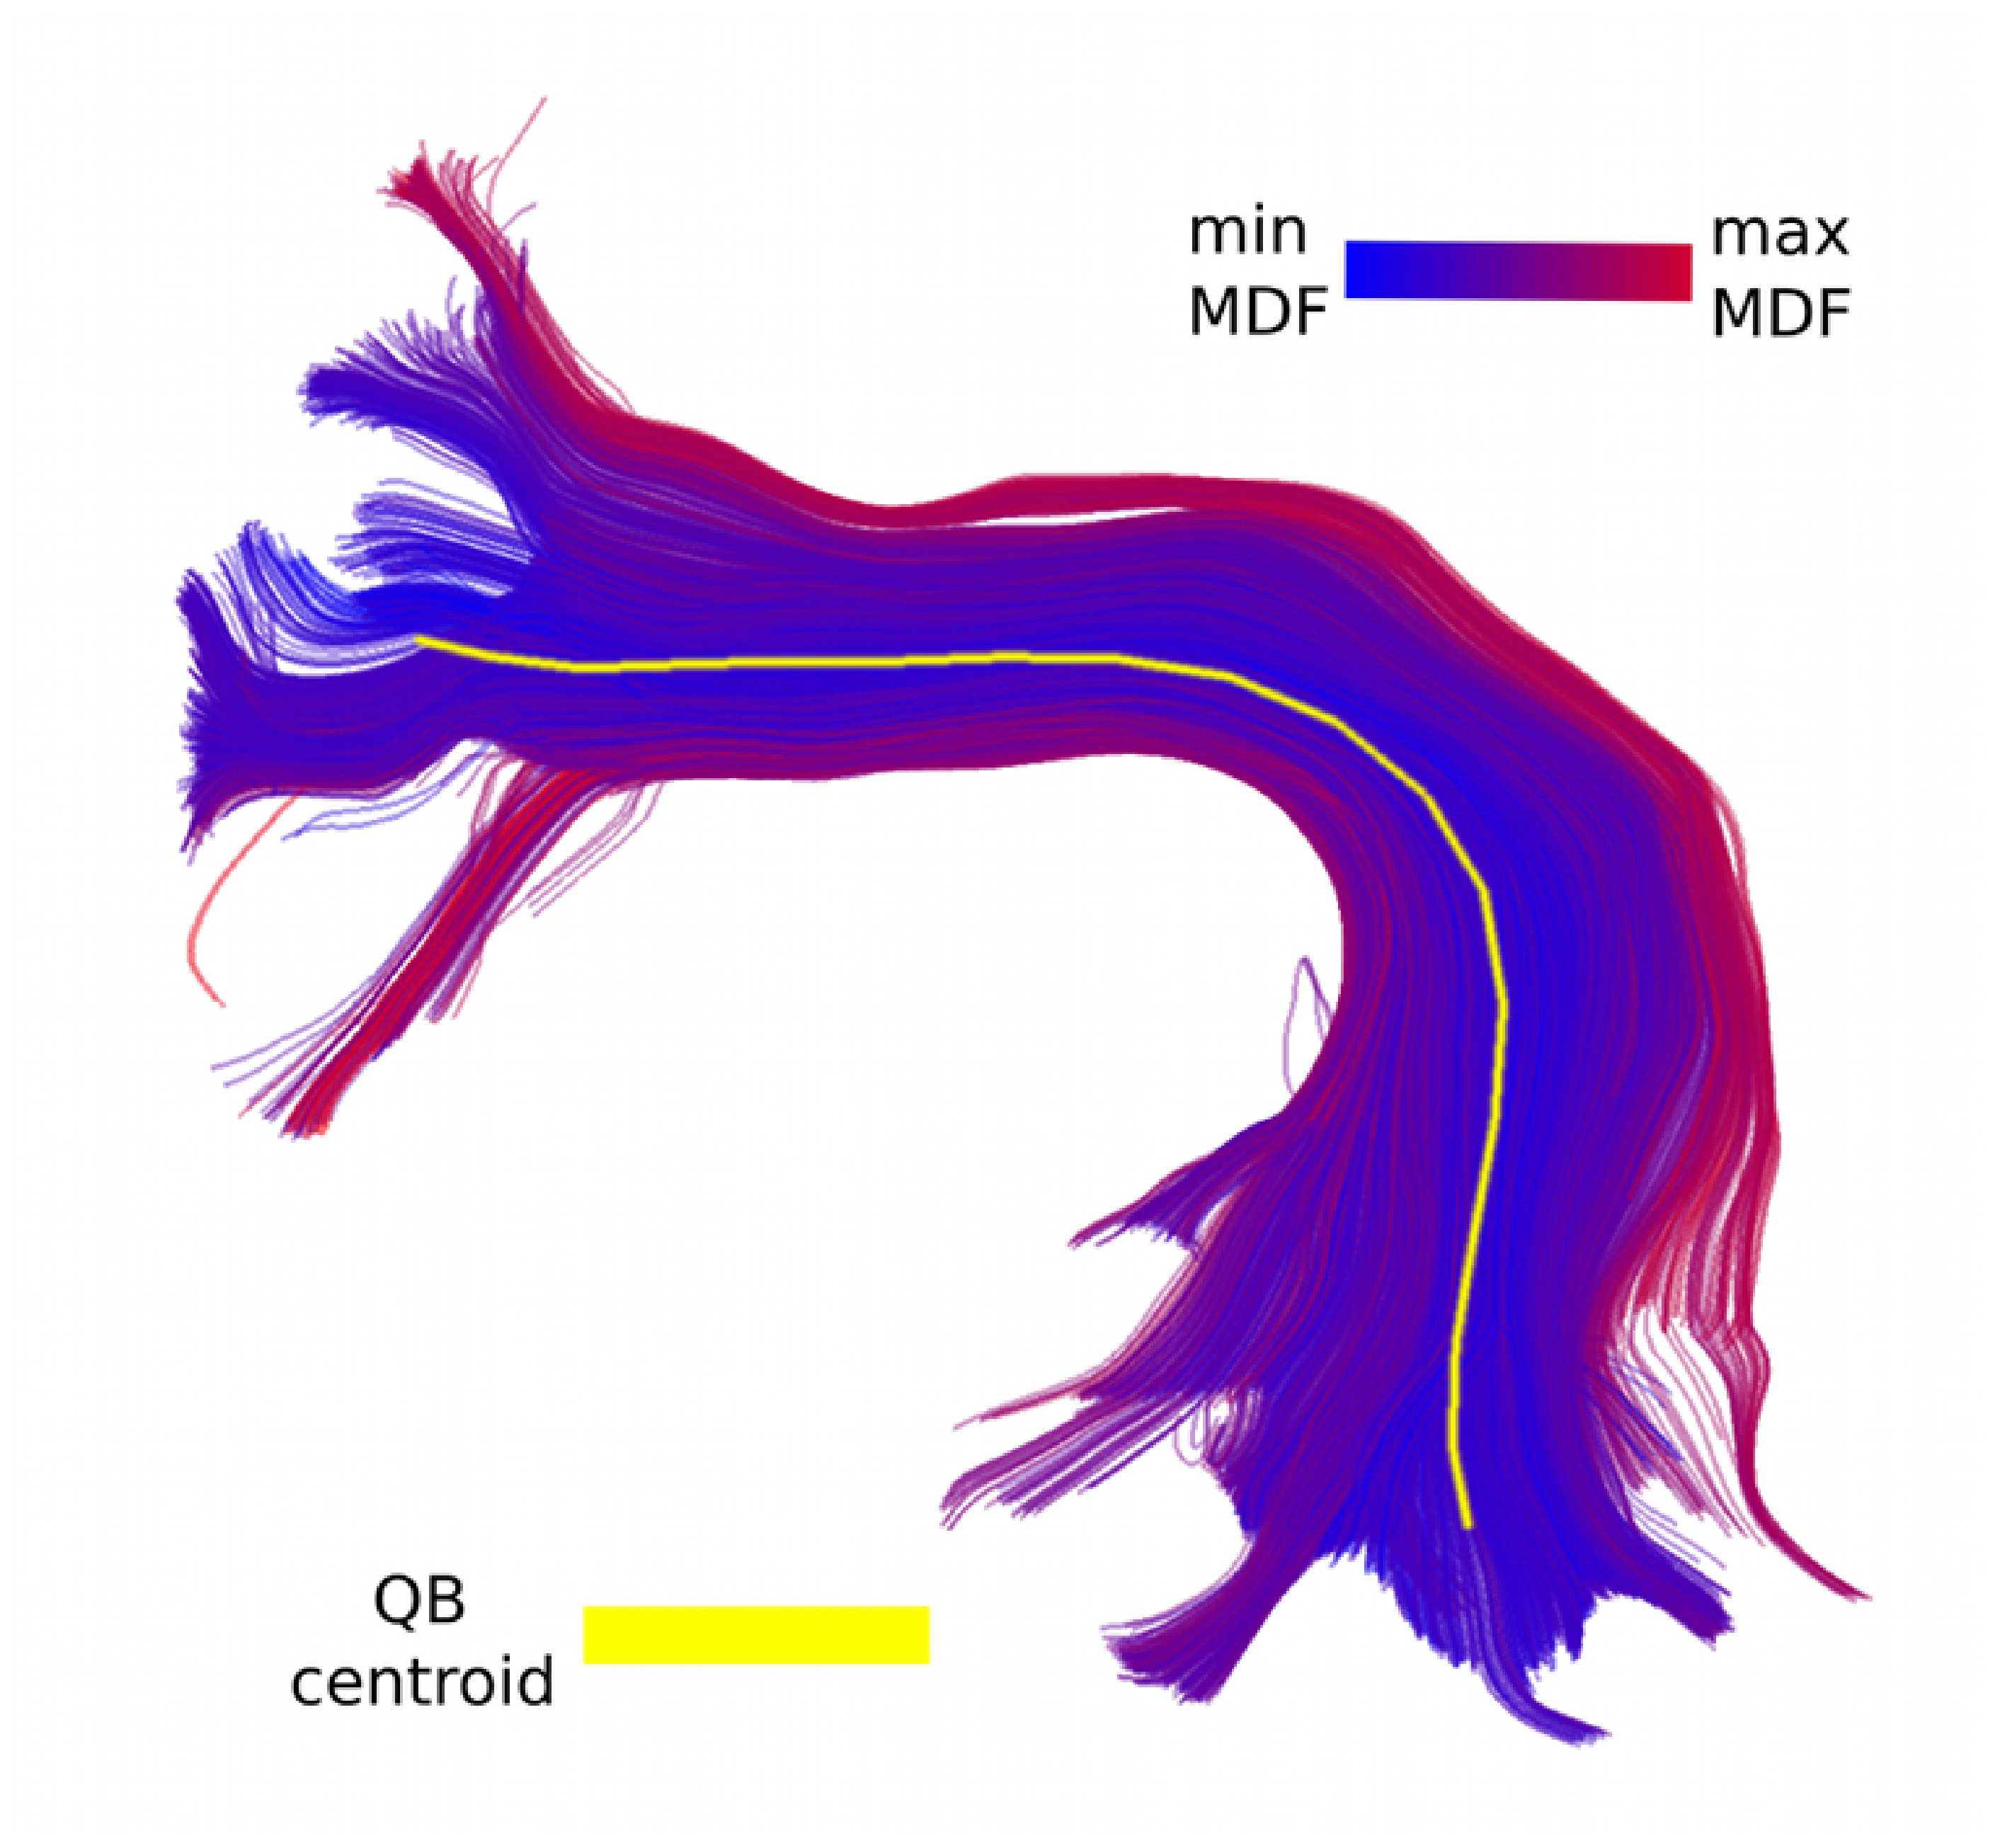
\includegraphics[scale=0.15]{Figures/Fig_11_MDF_arcuate}
\centering{}
\caption{Color coding shows MDF distances from QB centroid to every
  other track in the bundle.\label{Fig:little_picture}}
\end{figure}

Here are some displayed equations (see Eq.~\ref{eq:direct_flip_distance}):
\begin{eqnarray}
  d_{\textrm{direct}}(s, t) = d(s, t) & = & \frac{1}{K}\sum_{i=1}^{K}|s_{i}-t_{i}|,\nonumber\\
  d_{\textrm{flipped}}(s, t) & = & d(s,t^F) = d(s^F,t),\nonumber\\
  \textrm{MDF}(s, t) & = & \min(d_{\textrm{direct}}(s, t), d_{\textrm{flipped}}(s, t))\label{eq:direct_flip_distance}.
\end{eqnarray}

Inline mathematics goes like this: $\frac{1}{K}\sum_{i=1}^{K}|s_{i}-t_{i}|$

Here we have an example of a table (see Table~\ref{Table_1}).

\begin{table}[th] \processtable{QB centroids performance compared with
random subsets\label{Table_1}} {\begin{tabular}{rrrr} %\hline Thresholds &
Comparison & Coverage \% (s.d.) & Overlap (s.d.) \\ \hline
\multirow{2}{*}{$10$~mm/$10$~mm} & QB Centroids & 99.96 (0.007) & 2.44
(0.08)\\ & Random & 90.49 (0.41) & 6.16 (0.55)\\ \hline
\multirow{2}{*}{$20$~mm/$20$~mm} & QB Centroids & 99.99 (0.004) & 3.54
(0.18)\\ & Random & 95.86 (0.62) & 6.81 (0.93)\\ \hline
\end{tabular}}{}
\end{table}

References go like this: in parentheses \citep{Garyfallidis_thesis, Mori1999}, and in running text \citet{Garyfallidis_thesis}.

And here is an example of how to add some code.

\begin{python}
from dipy.viz import fvtk
ren = fvtk.ren()
class Test(object):
  def __init__(self, a):
    pass
@parametric
def f(x):
  return x**2
for i in range(10):
  print f(i)
\end{python}



\selectlanguage{british}%
\bibliographystyle{apalike2}
%\bibliographystyle{plainnat}
%\bibliographystyle{IEEEabrv, IEEEtran}
%\bibliographystyle{IEEEtran}
%\bibliographystyle{elsarticle-harv}
\selectlanguage{english}
\bibliography{scilBibTex}

\end{document}
